\begin{frame}[c]
	\begin{center}
		\huge \color{blue} Applications
	\end{center}
\end{frame}

\begin{frame}[fragile]{Set-up}
\begin{itemize}
\item $n=100$ observations:
	\begin{itemize}
	\item $y_1,\dots, y_{50} \iidsim \Nc(4,1)$
	\item $y_{51}, \dots, y_{100} \iidsim \Nc(7,1)$
	\end{itemize}
\item Prior parameters for the Normal-NIG model:
	\begin{itemize}
	\item $\mu_0 = 5$ 
	\item $\lambda_0 = 1$
	\item $\alpha_0 = 2$
	\item $\beta_0 = 2$
	\end{itemize}

\item \verb|Neal8|
	\begin{itemize}
	\item $m=3$ 
	\item \verb|maxiter| $=20000$
	\item \verb|burnin| $=5000$
	\item $K=15000$ valid iterations
	\end{itemize}
\end{itemize}
\end{frame}

\begin{frame}[fragile]{Cluster estimation}


\begin{verbatim}
unsigned int cluster_estimate();
\end{verbatim}

$$ \hat{k} = \argmin_k \left \lVert D^{(k)} - \bar D \right\rVert_F^2= \argmin_k \sum_{i,j} \left( D^{(k)}_{ij} - \bar{D}_{ij}  \right)^2$$


\begin{itemize}

\item $D^{(k)}$: dissimilarity matrix  at iteration k \\

\item $\bar D= \frac{1}{K} \sum_k D^{(k)} $: mean over $K$ iterations
\end{itemize}

\end{frame}

\begin{frame}[fragile]{Density estimation}


\begin{verbatim}
void eval_density(const std::vector<double> grid);
\end{verbatim}

\begin{equation}
	\begin{aligned} \nonumber
	\hat f^{(k)}(x) \ = \ \sum_j \frac{n^{(k)}_j}{M+n} f\left(x | \phi^{(k)}_j\right) \ + \ \frac{M}{M+n} m(x)
	\end{aligned}
\end{equation}

\begin{equation}
	\begin{aligned} \nonumber
		\hat m(x) = \frac{1}{m} \sum_{h=0}^{m-1}  f\left(x | \phi_h\right)
	\end{aligned}
\end{equation}

\begin{equation}
	\begin{aligned} \nonumber
 \Longrightarrow \hat f(x) = \frac{1}{K} \sum_k \hat f^{(k)}(x) 
\end{aligned}
\end{equation}

\end{frame}

\begin{frame}[c]
	\begin{center}
		\huge \color{blue} Results
	\end{center}
\end{frame}



\begin{frame}{Oscillations}
\begin{figure}[h]
	\centering
	\begin{minipage}{0.5\textwidth}
		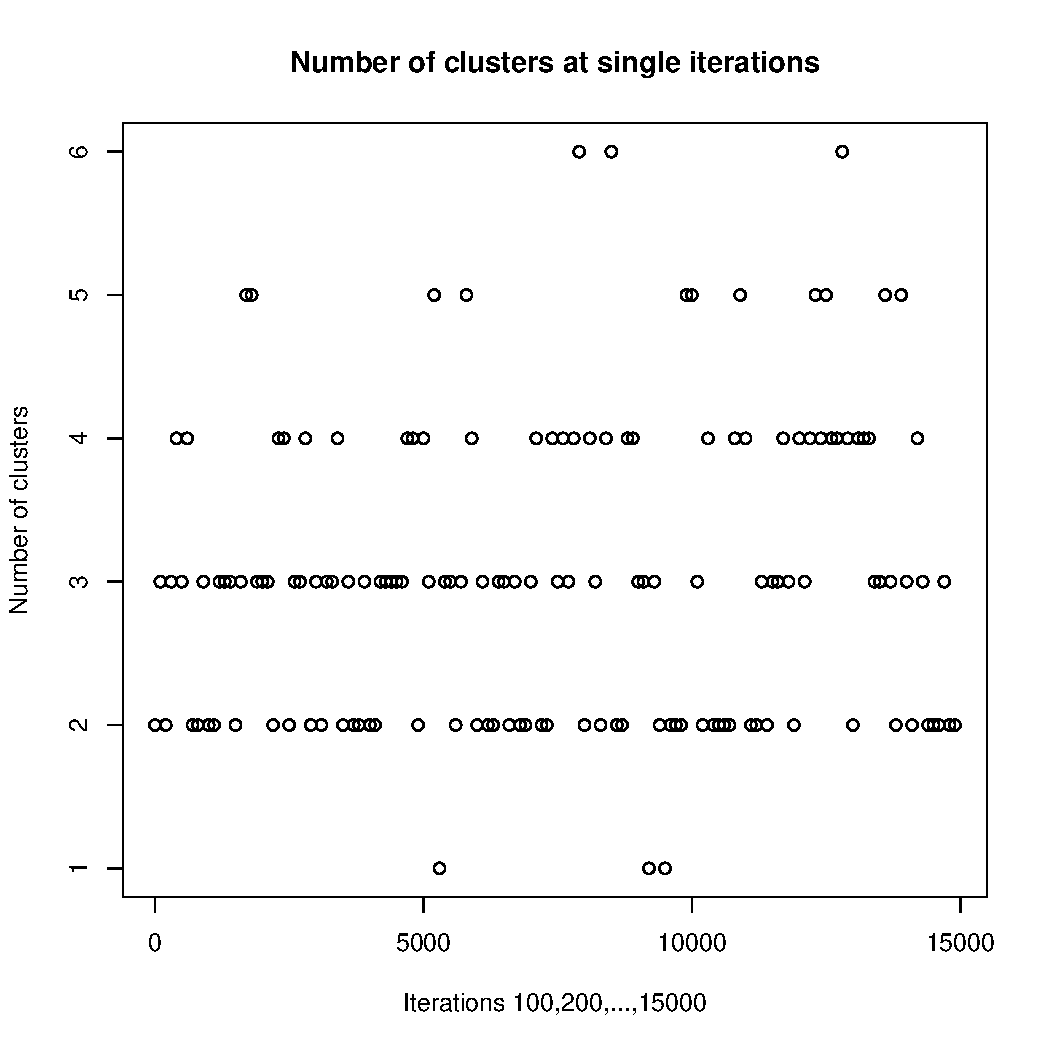
\includegraphics[scale=0.35]{etc/cardinalities_thinned.pdf}
	\end{minipage}%
	\begin{minipage}{0.5\textwidth}
		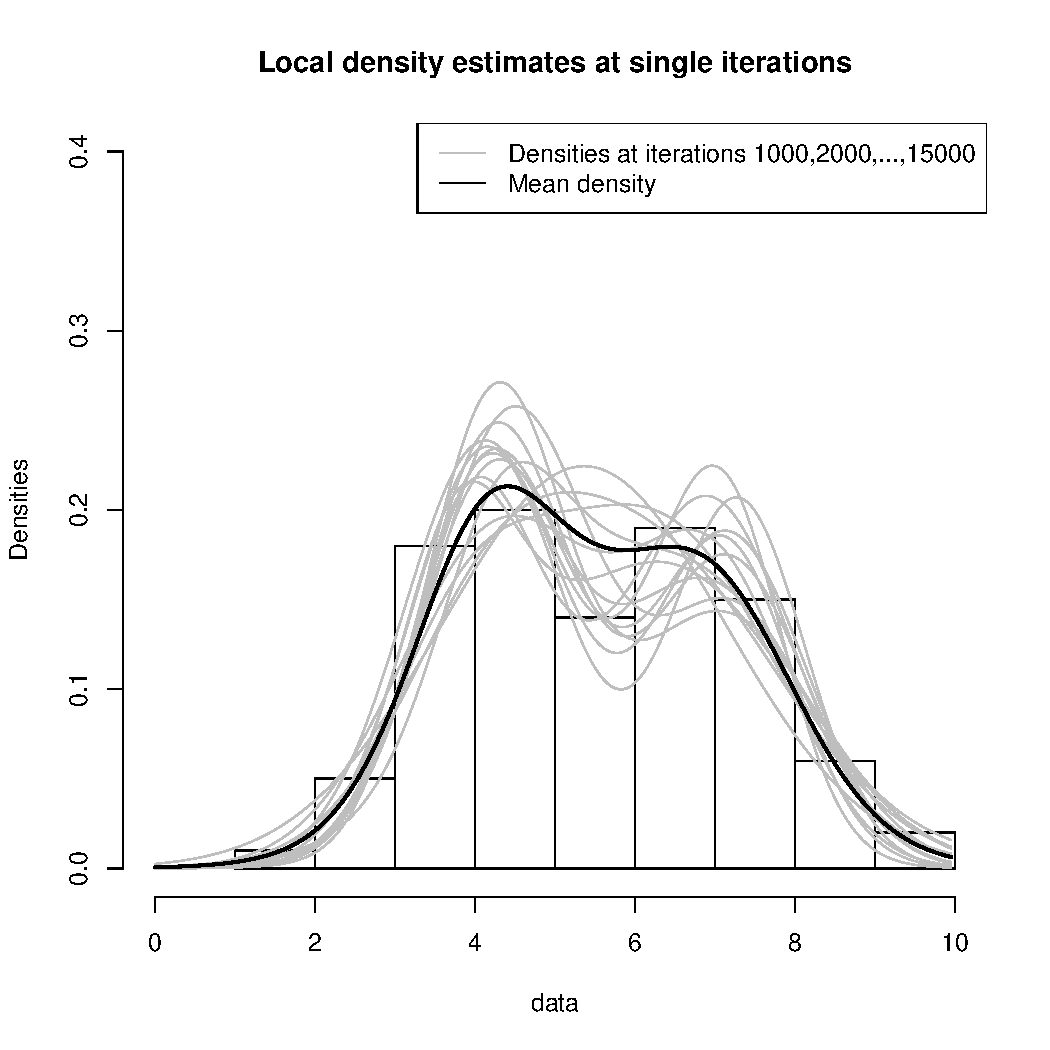
\includegraphics[scale=0.35]{etc/densities_iters.pdf}
	\end{minipage}
\end{figure}

\end{frame}

\begin{frame}{Total mass}

\begin{center}
		%\texttt{}
		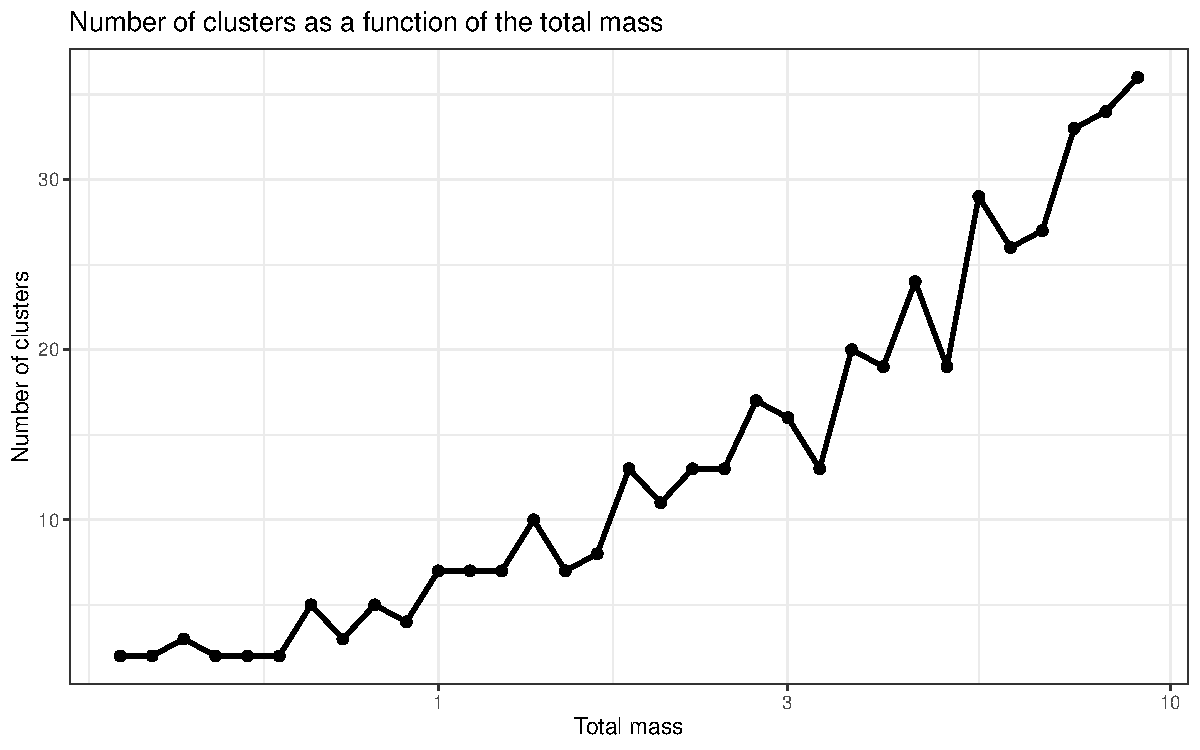
\includegraphics[scale=0.35]{etc/num_clust_M.pdf}
	\end{center}


\begin{center}
		%\texttt{a}
		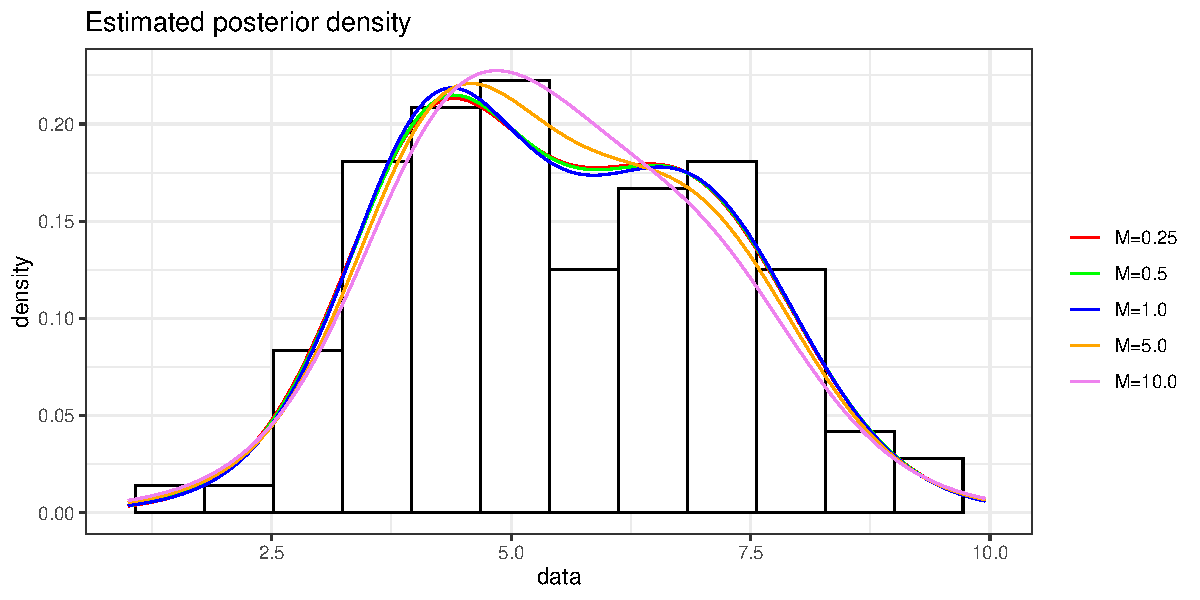
\includegraphics[scale=0.35]{etc/dens_withMm3.pdf}
	\end{center}
\end{frame}



\begin{frame}{Auxiliary parameters}

\begin{center}
		%\texttt{a}
		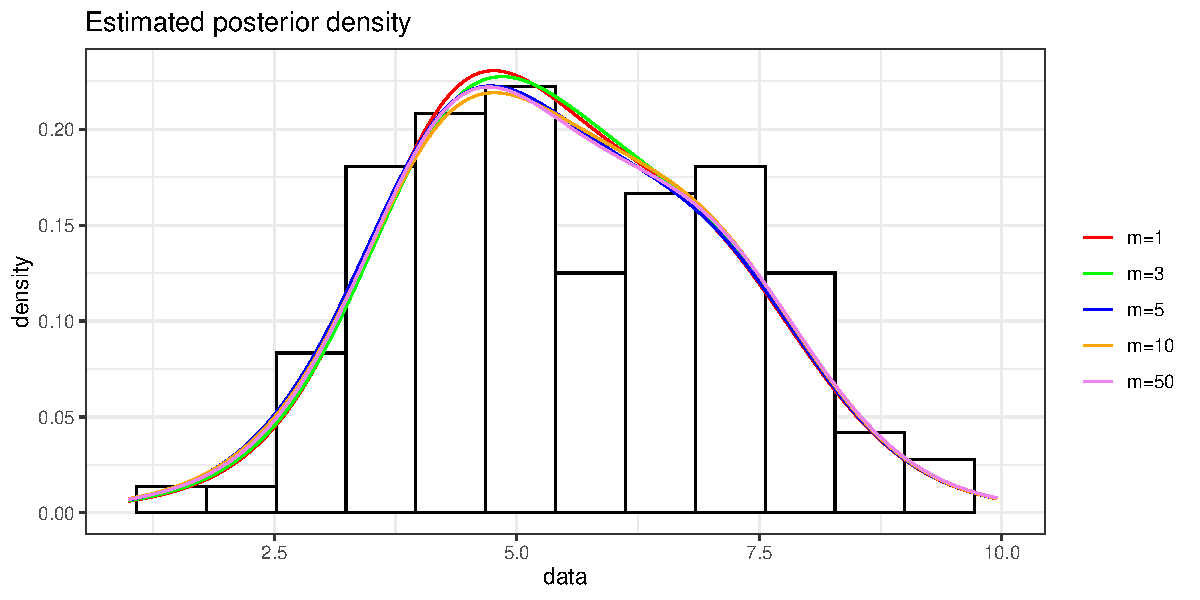
\includegraphics[scale=0.5]{etc/dens_withmM10.pdf}
	\end{center}
\end{frame}


\begin{frame}{Density components}

\begin{center}
		%\texttt{}
		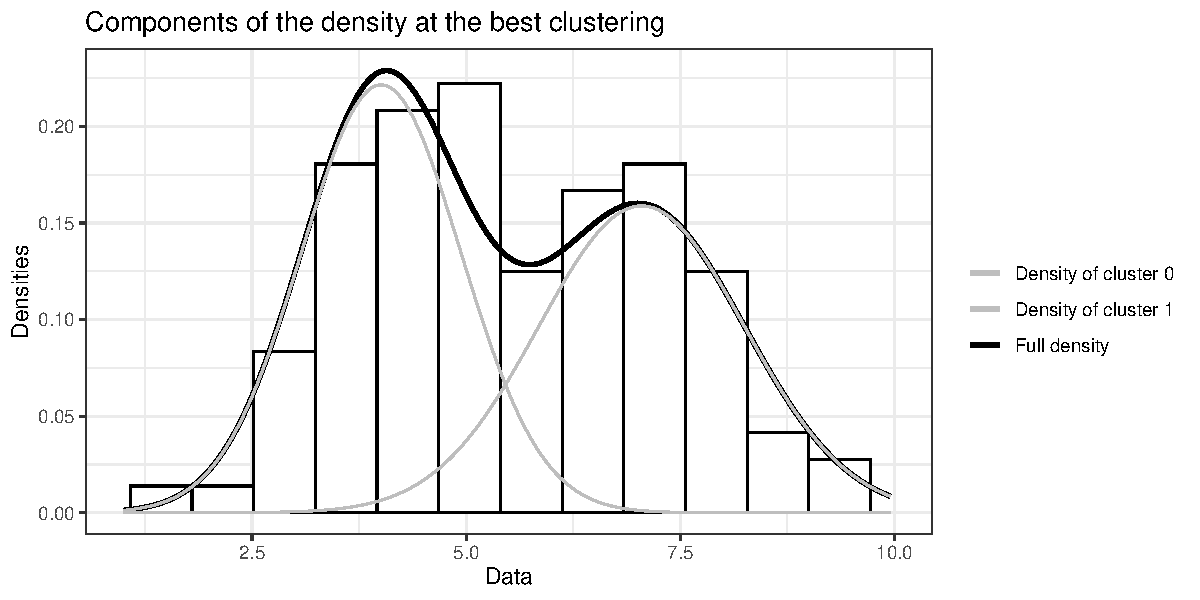
\includegraphics[scale=0.6]{etc/componentsM025m3_best.pdf}
	\end{center}
\end{frame}


\begin{frame}{Clustering}

\begin{center}
		%\texttt{a}
		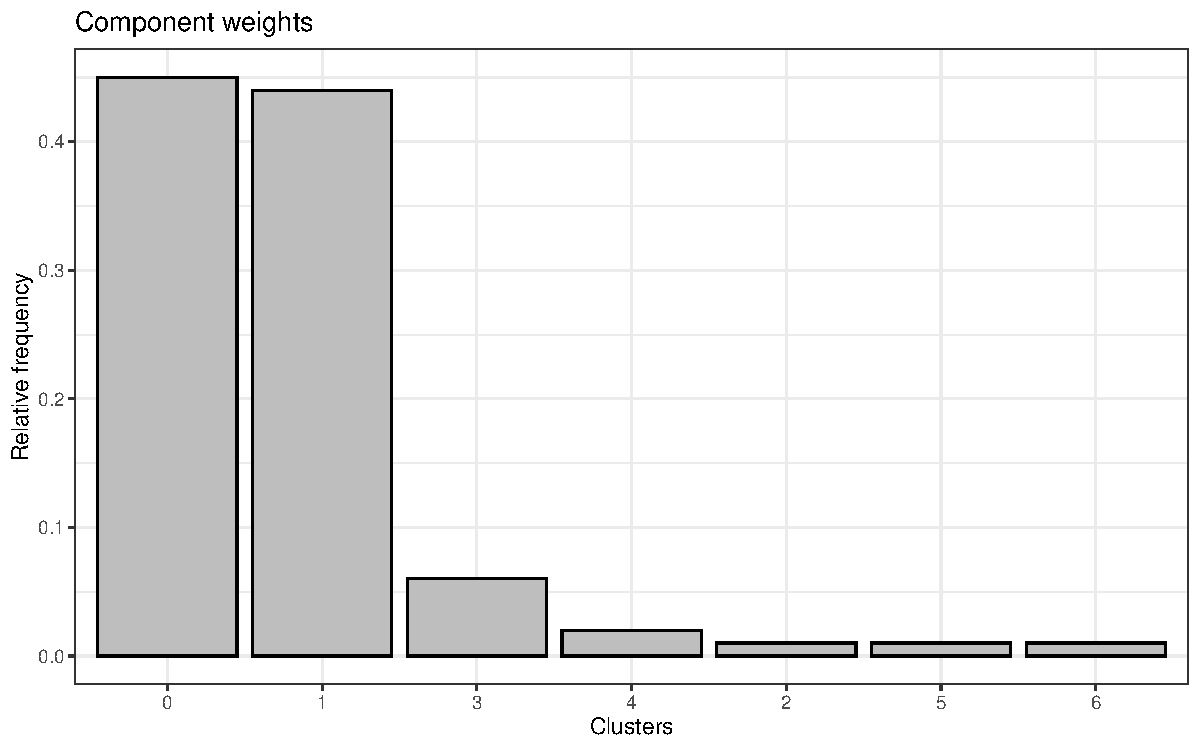
\includegraphics[scale=0.5]{etc/barplotM1m3.pdf}
	\end{center}
\end{frame}



\begin{frame}{\texttt{Neal2} vs \texttt{Neal8}}

\begin{center}
		%\texttt{a}
		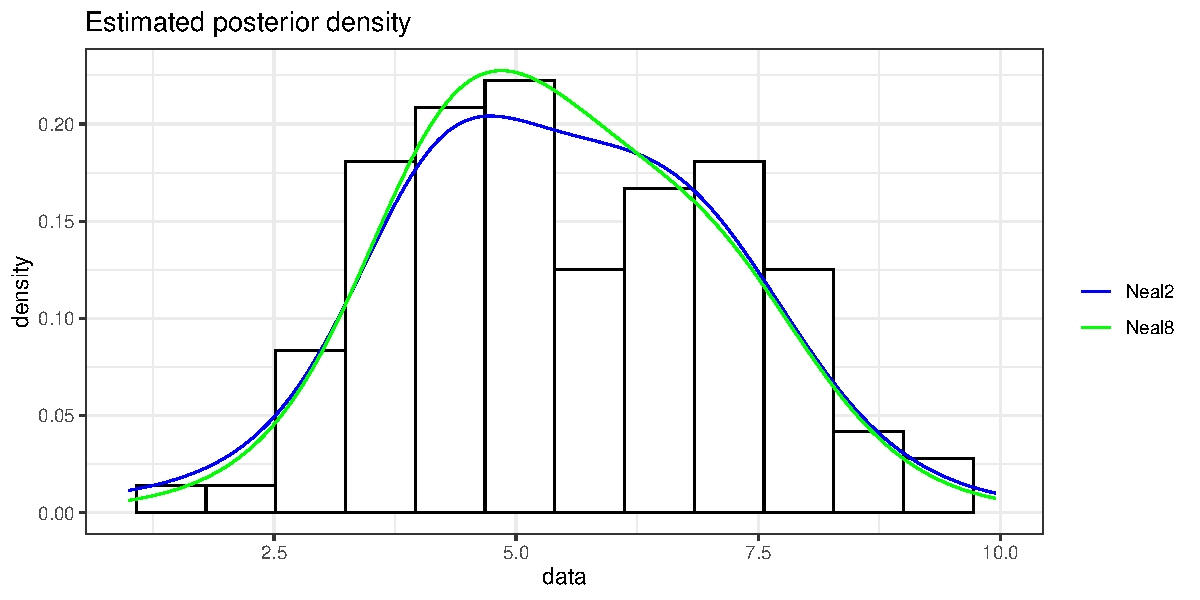
\includegraphics[scale=0.5]{etc/neal2_M10.pdf}
	\end{center}
	
\end{frame}


\begin{frame}[fragile]{Extensions}

	\begin{itemize}
	\item Adaptation to \verb|Hypers| containing hyper-priors
	\item Implementation of other \verb|Hierarchy| classes
	\item Adaptation to other \verb|Mixture| classes
	\item Interface with R and Python
	\item Integration of conjugacy-dependent algorithms to handle non-conjugacy
	\item Full generalization
	\end{itemize}

\end{frame}
